\chapter{固溶体}
    \section{固溶体}
        根据相的结构和形成条件,可以分成三种,固溶体、有序固溶体和金属
        间化合物;很具合金相在相图中的位置,可以将合金相分为纯金属、固溶体
        和金属间化合物。

        本章关注的重点是固溶体,固溶体是指不同元素的原子能够以变动的比例去占据晶体结构
        的位置(点阵)。即固溶体可以在一定的成分范围内存在,性能随成分变化而连续变化。
        固溶体溶解度的极限也称为固溶度。

        不同金属和化合物的固溶度差别很大,可以从几乎不溶解到完全互溶。固溶体
        可以无序,即组元在点阵中随机分布;也可以有序,即异类原子有规则的排列。有序可以是短程的,
        也可以是长程的。

        \subsection{固溶体及其类型}
            有些组元合金化后能形成一系列的固溶体:
            \begin{enumerate}
                \item \textbf{一次固溶体}\index{一次固溶体}:在含有金属组元的二元相图中,靠近金属组元的一端,一般总会有溶解度不同的固溶体,其晶体结构与溶剂金属相同,也被称为\textbf{边际固溶体}\index{一次固溶体!边际固溶体};
                \item \textbf{二次固溶体}\index{二次固溶体}:在相图的中间位置,晶体结构不一定与溶剂相同,又叫\textbf{中间相}\index{二次固溶体!中间相},即以化合物为基的固溶体。其中为长程序的中间相,称为\textbf{金属间化合物}\index{二次固溶体!金属间化合物}。
            \end{enumerate}

            根据溶质原子在晶体点阵的位置,可将固溶体分为三类:
            \begin{enumerate}
                \item 置换型:原子大小相近;
                \item 间隙型:原子尺寸差别较大;
                \item 缺位型:格点上某一类原子出现空缺。
            \end{enumerate}
        \subsection{影响固溶度的因素}
            影响固溶度的因素主要有三种,分别是尺寸因素、电子浓度因素和
            化学亲和力因素。
            \subsubsection{尺寸因素}
                若形成合金的组元的原子尺寸差超过14-15\%时,尺寸因素将会产生较大影响,
                使固溶度降低;容尺寸差小于15\%,尺寸因素成为次要的影响因素,固溶度由其他影响因素确定。
                这也就是Hume-Rothery规律\index{Hume-Rothery规律}。

                原子大小一般在\si{\angstrom},不同情况下,测得的原子大小不同,比如
                $\alpha-$\ce{Fe}和$\gamma-$\ce{Fe},原子的配位数分别为8和12,配位数越小,
                原子尺寸越小,所以$\alpha-$\ce{Fe}原子小于$\gamma-$\ce{Fe}。

                当异类原子形成固溶体时,符合Vegard定律,也就是粒子晶体电子常数$a$与固溶体成分$x$
                有线性关系:
                \begin{equation}
                    a=a_1+(a_2-a_1)x=a_1(1-x)+a_2x,
                \end{equation}
                其中$a_1$是溶剂的点阵常数,$a_2$是溶质的点阵常数。然而金属固溶体都或多或少偏离
                离子晶体,故也偏离Vegard定律,有的出现正偏差,有的出现负偏差。
            \subsubsection{电子浓度因素}
                电子浓度\index{电子浓度}是指价电子数和原子数的比值,记做$e/a$
                如果溶质原子的百分数为$x$,原子价为$v$,而溶剂的原子价为$V$,则合金的电子浓度为
                \begin{equation}
                    \frac{e}{a}=\frac{v x+(100-x) V}{100}.
                \end{equation}

                电子浓度对于原子是不确定的,由于原子“价”是不固定的。比如,一般认为
                \ce{Zn}是$+2$价,但已经证明,$+1$价电子完全贡献出来,第二个电子并不完全贡献
                出来,而仍有一定几率绕\ce{Zn}原子核转动,所以\ce{Zn}的价不是$+2$。
            \subsubsection{化学亲和力因素}
                原子的第一电离能\index{第一电离能}$E_I$是气态原子失去一个电子成为气态的
                一价正离子所需的能量,
                \begin{equation}
                    E_I=E(M^+)-E(M),
                \end{equation}
                其中$M$为原子。

                原子的电子亲合能$Y$是原子获得一个电子成为一价负离子
                时所放出的能量,即
                \begin{equation}
                    -Y=E_(M^-)-E(M),
                \end{equation}
                电子亲合能和第一电离能都可以通过实验测定。

                而A、B两原子形成$\mathrm{A}^{-}\mathrm{B}^{+}$必须满足
                \begin{equation}
                    E_{IA}+Y_{A}>E_{IB}+Y_{B},
                \end{equation}
                以$E_I+Y$表示\textbf{化学亲合力}\index{化学亲和力},通常称之为\text{负电性}\index{负电性}。
                它表示组元吸引电子的能力。负电性越大的组元,吸引电子的
                能力也越强。形成离子化合物时,负电性大的元素成为负离子,负电性小的成为正离子。

                实际只需负电性的相对大小,人为规定氟的负电性为4.0。负电性有周期性。但贵金属\ce{Cu}、\ce{Ag}、
                \ce{Au}是例外。负电性概念比较适用于金属间化合物。
        \subsection{固溶体自由能的统计理论}
            根据共晶型相图\autoref{CuAg相图},BC和GH分别代表组元B在A中和A在B中的溶解度曲线,实际上就是在不同温度下的浓度曲线$c(T)$
            \begin{figure}[ht]
                \centering
                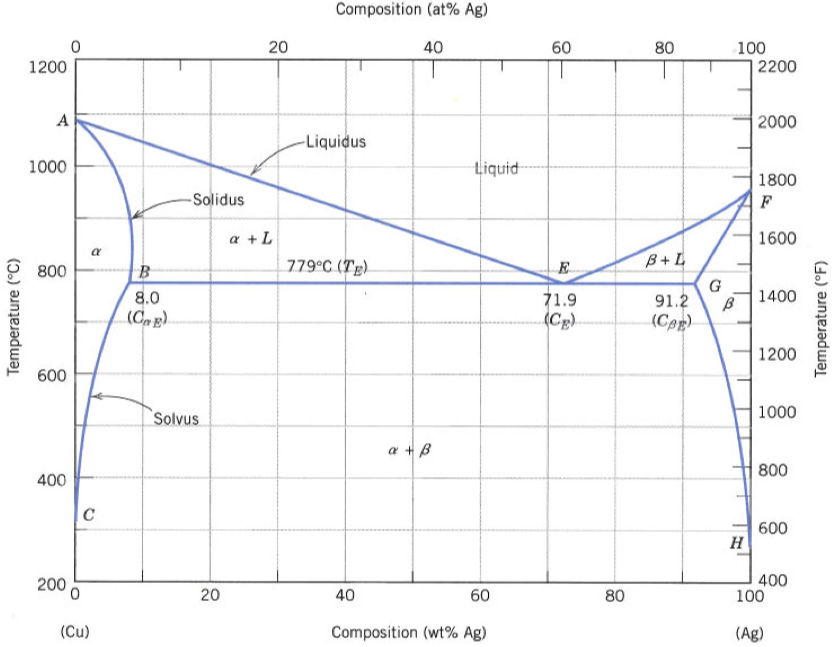
\includegraphics[width=0.7\textwidth]{fig/Cu_Ag_Phase_Diagram.png}
                \caption{\ce{Cu}和\ce{Ag}的相图,图片来源:\href{http://resource.npl.co.uk/mtdata/phdiagrams/agcu.htm}{National Physical Laboratory}。}
                \label{CuAg相图}
            \end{figure}

            要求解浓度$c(T)$,及必须先求解体系自由能$F(c,T)$,再利用相平衡求出$c(T)$,即
            固溶度方程。

            在求解自由能时需要用到准化学近似\index{准化学近似},假定固态原子之间存在化学键,因而晶体的
            内能可以按拆散或形成的键数用统计方法加以计算。假设A、B组元形成置换固溶体,原子浓度
            分别为$(1-c)$和$c$,假设原子总数为$N$,则有
            \begin{align}
                N_A&=N(1-c)=N-n,\\
                N_B&=Nc=n.
            \end{align}
            自由能为
            \begin{equation}
                F=E-TS,
            \end{equation}
            因此,应当先表示体系的内能和熵。假设固溶体在\SI{0}{\K}的内能为$E_0$,比热为
            $C_p$,则在$T$时的内能和熵为
            \begin{align}
                E&=E_0+\int_{0}^{T}C_p\dif T,\\
                S&=\Delta S_{\mathrm{m}}+\int_{0}^{T}\frac{C_p}{T}\dif T.
            \end{align}
            式中$\Delta S_{\mathrm{m}}$为混合熵:
            \begin{equation}
                \Delta S_{\mathrm{m}}=k\left( \ln\omega_{AB}+\ln\omega_{A}+\ln\omega_B \right)\label{固溶体系的混合熵}.
            \end{equation}
            在热力学上,单质的组态熵为零,因此$\omega_A=\omega_B=1$,而固溶体的组态熵为
            \begin{equation}
                \omega_{AB}=\frac{N!}{N_A!N_B!}=\frac{N!}{n!(N-n)!},
            \end{equation}
            代入\autoref{固溶体系的混合熵}可得
            \begin{equation}
                \Delta S_{\mathrm{m}}=k\ln\frac{N!}{n!(N-n)!},
            \end{equation}
            利用Stirling近似,可得
            \begin{equation}
                \Delta S_{\mathrm{m}}=k[N\ln N-n \ln n-(N-n) \ln (N-n)],
            \end{equation}
            因为$c=n/N$,$1-c=(N-n)/N$,所以变成
            \begin{equation}
                \Delta S_{\mathrm{m}}=-N k[c \ln c+(1-c) \ln (1-c)],
            \end{equation}
            由于浓度均小于1,所以$\Delta S_{\mathrm{m}}>0$。

            对于内能的求解则从结合能出发,假设A、B形成固溶体是,晶体中无缺陷,原子紊乱分布,
            则晶体中存在三种键AA、BB和AB的个数分别为
            \begin{align}
                N_{AA}&=\frac{1}{2}N(1-c)\cdot(1-c)\cdot Z,\\
                N_{B B}&=\frac{1}{2} N c \cdot c \cdot Z,\\
                N_{A B}&=N c \cdot(1-c) \cdot Z.
            \end{align}
            原子间作用能用$V$表示,内能$E_0$等于合金中所有最近邻原子间作用能之和
            \begin{equation}
                \begin{aligned}
                    E_{0}&=V_{A A} N_{A A}+V_{B B} N_{B B}+V_{A B} N_{A B}\\
                    &=\frac{1}{2} N Z\left[(1-c)^{2} \cdot V_{A A}+c^{2} \cdot V_{B B}+2 c(1-c) \cdot V_{A B}\right]\\
                    &=\frac{1}{2} N Z\left[c V_{B B}+(1-c) V_{A A}+c(1-c)\left(2 V_{A B}-V_{A A}-V_{B B}\right)\right].
                \end{aligned}\label{固溶体内能与成键关系的一般表达式}
            \end{equation}
            前两项为纯A和纯B的内能,第三项为固溶后内能的改变量$\Delta E$。
            固溶体的形成能为
            \begin{equation}
                \Delta E=NZc(1-c)V=N_{AB}V,
            \end{equation}
            其中$V=V_{AB}-\frac{1}{2}(V_{AA}+V_{BB})$为形成一个AB键时内能的改变量。
            
            不考虑随温度带来热容变化,计算得到的自由能为
            \begin{equation}
                \begin{aligned}
                    F&=E-TS\\
                    &=E_0+\int_{0}^{T} C_{\mathrm{p}} \mathrm{d} T-T\left(\Delta S_{\mathrm{m}}+\int_{0}^{T} \frac{C_{\mathrm{p}}}{T} \mathrm{d} T\right)\\
                    &=K(c, T)+\frac{1}{2} N Z\left[c V_{\mathrm{BB}}+(1-c) V_{\mathrm{AA}}\right]+N Z c(1-c) V\\
                    &+N k T[c \ln c+(1-c) \ln (1-c)].
                \end{aligned}\label{固溶体自由能的表达式}
            \end{equation}
            影响自由能曲线的有两部分$V$和$T\Delta S_m$,因此按照$V=0$、$V<0$和$V>0$可以分为三种情况:
            \begin{enumerate}
                \item[1] $V=0$,即形成固溶体时能量不变,固溶体是理想固溶体,$E_0$为浓度的线性方程,自由能有极小值,不论合金成分如何都会形成单相固溶体;
                \item[2] $V<0$,虽然$E_0$不再是直线,但是也形成单相固溶体;
                \item[3] $V>0$,自由能曲线存在两个拐点\footnote{拐点为二阶导数为零的点。},也就是在这两个拐点之间,体系分解为两相混合物。
            \end{enumerate}

            在计算$E_0$时作出了两个主要的假定:
            \begin{enumerate}
                \item[1] 原子随机分布假定:
                \begin{enumerate}
                    \item 然而只有形成固溶体的内能不变,也就是$V=0$时,内能分布才和原子分布无关,原子才能随机分布;
                    \item 当$V<0$时,形成AB键使内能下降,合金倾向与形成更多的AB键,也就是异类原子相互吸引,此时公式中的$N_{AB}$偏小,但是对内能和熵的影响可以相互补充,对结果影响不大;
                    \item 同理,$V>0$时,对自由能和熵的影响也是相互补偿的,对结果影响不大;
                \end{enumerate} 
                \item[2] 最近邻原子键能的假定:计算$E_0$是,认为它等于合金中所有最近邻原子间作用能之和,但是
                \begin{enumerate}
                    \item 侧重考虑化学亲和力因素,忽略了键所处的环境;
                    \item 当电子浓度因素起主要作用时,价电子属于整个晶体,并不构成定向键;
                    \item 当尺寸因素起主要作用时,畸变能牵涉到若干原子间距,这与研究的体系相关。
                \end{enumerate} 
            \end{enumerate}
        \subsection{固溶度方程}
            假设各个原子之间的结合能相等,各组分的热容也相等,在$N=N_0$也就是\SI{1}{\mol}分子
            的情况下,\autoref{固溶体自由能的表达式}可以写作
            \begin{equation}
                F=K(T)+\frac{1}{2}N_{0} Z V_{0}+N_{0} Z V c(1-c)+N_{0} k T[c \ln c+(1-c) \ln (1-c)].
            \end{equation}
            平衡条件为
            \begin{equation}
                \frac{\dif F}{\dif c}=0,
            \end{equation}
            因此
            \begin{equation}
                \frac{\dif F}{\dif c}=N_{0} Z V(1-2 c)+R T[\ln c-\ln (1-c)]=0.
            \end{equation}
            解得
            \begin{equation}
                \frac{c}{1-c}=\exp \left[-\frac{\mathrm{N}_{0} Z V(1-2 c)}{R T}\right],
            \end{equation}
            这就是固溶度方程\index{固溶度方程}。

            当固溶度浓度很小时,$1-c\simeq 1$,$1-2c\simeq 1$,此时固溶度方程为
            \begin{equation}
                c=\exp \left(-\frac{N_{0} Z V}{R T}\right)\label{低浓度固溶度方程},
            \end{equation}
            所以在固溶度不大的系统中,随温度升高,溶解度增大,且与温度有指数关系。

            形成固溶体时内能该变量为
            \begin{equation}
                \Delta E=N_0Zc(1-c)V=N_{AB}V,
            \end{equation}
            对$c$求微分,得到
            \begin{equation}
                \frac{\dif \Delta E}{\dif c}=N_0ZV(1-2c)\simeq N_0ZV,
            \end{equation}
            其中认为固溶体浓度很小,采用了$1-2c\simeq 1$的近似。

            在恒温恒压过程中,
            \begin{equation}
                N_0ZV\simeq \Delta\bar{H}_B,
            \end{equation}
            其中$\Delta\bar{H}_B$为溶解热,表示在无限大固溶体中加入单位纯组元B的焓变,
            这是可以测量的物理量。所以\autoref{低浓度固溶度方程}可以写作
            \begin{equation}
                c=\exp \left(-\frac{\Delta \overline{H}_{B}}{R T}\right).
            \end{equation}

        %\subsection{固溶体的物理性能}
    \section{有序固溶体}
        形成有序固溶体的驱动力是形成固溶体的内能变化$V<0$,另一个条件是两个组元有
        有合适的比例。然而在形成过程中,组态熵随固溶体的有序度增加而下降,这会对有
        序固溶体的形成造成阻力。

        在一定的温度范围内,可能发生有序-无序转变,也就是第二类相变。一般是不同原子在结合
        后的能量低于未结合的能量时发生。在高温下,有序的小原子群
        不断地形成和消失,在冷却过程中,短程有序得到更大的发展。达到临界温度$T_c$时,这些
        小原子群长大,形成有序畴\index{有序畴}。如果相邻的有序畴是反向的,这被称为反向畴\index{反向畴}。
        由于体系倾向与不同原子成键,因此在畴内同种原子之间几乎不成键,只有在畴界面上才会成键,如\autoref{畴界面上原子}所示。

        \begin{figure}[ht]
            \centering
            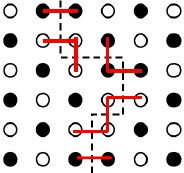
\includegraphics[width=0.5\textwidth]{fig/bands_near_domian_boundry.jpg}
            \caption{在畴界面上原子的成键情况,其中同种原子成键仅有9对,异种原子成键有51对。}
            \label{畴界面上原子}
        \end{figure}

        温度低于临界温度$T_c$时,畴壁不再稳定,反向畴吞并长大,长程有序,成为超结构\index{超结构}。
        \num{1e4}个原子以上时,会出现超结构线条。


        \subsection{有序固溶体的晶体结构}
            有序性随温度的变化而变化,当温度高于临界温度$T_c$时,体系的内能增加,根据
            \begin{equation}
                F=E-TS,
            \end{equation}
            想要使体系的自由能降低,体系必须向熵增的方向发展,因此结构也就会逐渐无序化。    
            在临界温度以下,有序结构可以存在一定成分范围内,只有特定成分才能达到完全有序。
            实际的有序化还分为长程有序和短程有序。
        \subsection{有序度参数}
            假设体系中$N_{AB}$为$AB$键的数目,定义短程序参数
            \begin{equation}
                \alpha_1=1-\frac{N_{AB}}{N_{AB}^*},
            \end{equation}
            当形成AB键的能量小于形成相同数量AA键和BB键的能量时,$V<0$,此时$N_{AB}>N^*_{AB}$,$\alpha_1<0$,
            为短程序状态;当$V=0$时,$\alpha_1=0$,是完全无序状态;当$V>0$时,$\alpha_1>0$,
            是同类原子偏聚状态。

            这一参数虽然能够描述体系的短程有序化程度,但是在短程序时,参数为负值,这对实际
            使用造成了障碍,因此Bethe引入了另一个短程序参数$\sigma$,定义为
            \begin{equation}
                \sigma=\frac{N_{A B}-N_{A B}^{*}}{\left(N_{A B}\right)_{\max }-N_{A B}^{*}},
            \end{equation}
            其中$\left( N_{AB} \right)_{\mathrm{max}}$为完全有序时AB键的个数。当体系完全有序时,
            $\sigma=1$;完全无序时,$\sigma=0$。

            在定义长程序参数之前,先假设格点分为$\alpha$、$\beta$两类,其中A原子占据
            $\alpha$格点位置,B原子占据$\beta$位置。令A原子占据某一$\alpha$位置的几率为
            $P_A^\alpha$,则长程序参数$\phi$定义为
            \begin{equation}
                \varphi=\frac{P_{A}^{\alpha}-C_{A}}{1-C_{A}}=\frac{P_{B}^{\beta}-C_{B}}{1-C_{B}}\label{长程序参数},
            \end{equation}
            其中$P_A^\alpha$、$P_B^\beta$分别是A、B原子占据$\alpha$、$\beta$点阵的几率。
            当体系完全有序时,$\phi=1$,体系完全无序时,$\phi=0$。
        \subsection{长程序的统计理论}
            以$\beta$黄铜为例,用准化学方法讨论其长程序。$\beta$黄铜是\ce{CuZn}合金,各占50\%at.,
            晶体为bcc结构,由两个互相穿插的简单立方点阵$\alpha$、$\beta$构成。

            当$c=\frac{1}{2}$时,根据\autoref{长程序参数},A原子处于$\alpha$位置和$\beta$位置的概率为
            \begin{align}
                P_{A}^{\alpha}&=\frac{1+\varphi}{2},\\
                P_{A}^{\beta}&=\frac{1-\varphi}{2},
            \end{align}
            同理可得B原子处于不同位置的概率。

            假设原子总数为$N$,则\ce{Cu}、\ce{Zn}各有$N/2$个,其中处于$\alpha$位置的
            A原子数目为$P_{A}^{\alpha} \cdot \frac{N}{2}=\frac{N}{4}(1+\varphi)$,
            处于$\beta$位置的A原子数目为$P_{A}^{\beta} \cdot \frac{N}{2}=\frac{N}{4}(1-\varphi)$,
            同理可得处于$\alpha$、$\beta$位置的B原子数目。

            以AA键为例,AA键的数目等于在$\alpha$位置上出现的$A$原子的概率乘以$\beta$位置上出现的
            A原子的概率乘以配位数。体系内AA、BB和AB键的数目分别为
            \begin{align}
                N_{A A}&=\frac{N}{4}(1+\varphi) \cdot \frac{1-\varphi}{2} \cdot Z=\frac{N Z}{8}\left(1-\varphi^{2}\right) \\
                N_{B B}&=\frac{N Z}{8}\left(1-\varphi^{2}\right) \\
                N_{A B}&=\frac{N}{4}(1+\varphi) \cdot \frac{1+\varphi}{2} \cdot Z+\frac{N}{4}(1-\varphi) \cdot \frac{1-\varphi}{2} \cdot Z=\frac{N Z}{4}(1+\varphi^2).
            \end{align}
            因而,内能与有序度$\varphi$的关系为
            \begin{align}
                E_{0}&=N_{A A} V_{A A}+N_{B B} V_{B B}+N_{A B} V_{A B} \\
                &=\frac{N Z}{8}\left[V_{A A}+V_{B B}+2 V_{A B}\right]+\frac{N Z}{8} \varphi^{2}\left[2 V_{A B}-V_{A A}-V_{B B}\right].
            \end{align}
            对于\autoref{固溶体内能与成键关系的一般表达式},当$c=\frac{1}{2}$时,可得
            \begin{equation}
                E_{0}=\frac{N Z}{8}\left[V_{A A}+V_{B B}+2 V_{A B}\right],
            \end{equation}
            当体系处于完全无序状态,也就是$\varphi=0$,两个内能表达式相同,因此有序化引起的内能该变量
            为
            \begin{equation}
                \frac{N Z}{8} \varphi^{2}\left[2 V_{A B}-V_{A A}-V_{B B}\right]=\frac{NZV}{4}\varphi^2,
            \end{equation}
            由于$V<0$,所以上式小于零,也就是\textbf{有序化使内能下降}。

            对于$\alpha$点阵内有$\frac{N}{2}$个位置,亚点阵有$N(1+\varphi)/4$个A原子,$N(1-\varphi)/4$个
            B原子,均为随机分布,所以$\alpha$亚点阵的组态数为
            \begin{equation}
                \omega_\alpha=\frac{\frac{N}{2} !}{\frac{N}{4}(1+\varphi) ! \frac{N}{4}(1-\varphi) !},
            \end{equation}
            同理$\omega_\beta=\omega_\alpha$,系统的组态数为
            \begin{equation}
                \omega=\omega_\alpha\cdot\omega_\beta,
            \end{equation}
            系统的混合熵为
            \begin{equation}
                \begin{aligned}
                \Delta S_{m}&=k \ln W \\
                    &=-N k\left[\frac{1+\varphi}{2} \ln \frac{1+\varphi}{2}+\frac{1-\varphi}{2} \ln \frac{1-\varphi}{2}\right].
                \end{aligned}
            \end{equation}
            当$\varphi=0$时,与以前讲固溶体自由能结果相同
            \begin{equation}
                \Delta S_{m}=-Nk\left( \frac{1}{2}\ln\frac{1}{2}+\frac{1}{2}\ln\frac{1}{2} \right),
            \end{equation}
            当$\varphi=1$时,体系完全有序,组态数只有1种,$\ln1=0$,体系熵为零,因此随有序度增加,熵值降低。

            体系的自由能为
            \begin{equation}
                F=\frac{N Z}{8}\left[V_{A A}+V_{B B}+V_{A B}\right]+\frac{N Z V}{4} \varphi^{2}+N k T\left[\frac{1+\varphi}{2} \ln \frac{1+\varphi}{2}+\frac{1-\varphi}{2} \ln \frac{1-\varphi}{2}\right],
            \end{equation}
            当$\frac{\dif F}{\dif \varphi}=0$时,
            \begin{equation}
                \frac{\dif F}{\dif \varphi}=\frac{1}{2} N Z V \varphi+\frac{N R T}{2} \ln \frac{1+\varphi}{1-\varphi}=0
            \end{equation}
            由此可以求出临界温度
            \begin{equation}
                T_c=-\frac{ZV}{2k},
            \end{equation}
            代入$\frac{\dif F}{\dif \varphi}=0$,得到
            \begin{equation}
                2\varphi\frac{T_c}{T}=\ln\frac{1+\varphi}{1-\varphi}
            \end{equation}
            也就是温度和有序化的关系。
        %\subsection{有序化对合金性能的影响}
    \section{中间相}
        已经发现的中间相\index{中间相}数以千计,键合性质各不相同,按控制形
        成化合物的因素分类可分为化学化合物、电子相和尺寸因素化合物三种。
        这里主要关注中间相成分、结构和性能的规律。但是由于目前的理论仍然是不完善的,
        因此只介绍重要的中间相,分别是正常价化合物、电子化合物、尺寸因素化合物和$\sigma$相(脆性相)。
        \subsection{电子化合物}
            根据Hume-Rothery规律,中间相\index{中间相!电子化合物}受电子浓度控制,
            可以在较宽的浓度区间内存在,它们的稳定性和电子浓度之比有关。
        \subsection{正常价化合物}
            由Zintl提出,\textbf{受电负性控制},,当二组元电负性差大时,容
            易形成。形成的成分范围窄,元素呈正常价。键合方式为离子键、
            共价键,如\ce{NaCl}等。
        \subsection{尺寸因素化合物}
            当两种元素的原子半径相差很少时,将形成电子化合物。当
            原子的半径相差很明显时,便形成尺寸因素化合物,并分为两种
            类型:间隙型、置换型。

            对于间隙型,当非金属原子对金属原子的半径比小于0.59时,金属原子构成fcc、bcc、hcp等简单结构,二非金属原子
            处于间隙位置,相具有相对简单的结构;而比值大于0.59时,形成复杂结构,而且存在畸变。
            间隙相具有金属性,可以存在于较宽的浓度区间内,比如$\ce{TiC_{0.6}}\sim\ce{TiC}$,$\ce{VC_{0.75}}\sim\ce{VC}$。

            对于中等原子尺寸差别,比如相差20\%到30\%之间,晶体结构为置换型,也就是Laves相\index{Laves相},
            则可以得到原子的有效堆积。Lavas相一般为$\mathrm{AB}_2$型,具有三种结构,分别为\ce{MgCu_2}立方结构型、
            \ce{MgZn_2}六角结构型和\ce{MgNi_2}六角结构型,其中小原子都排列在四面体的空间点阵上。
        \subsection{脆性相}
            最初在\ce{Fe}-\ce{Cr}系中被发现,使材料变脆,在一些高温合金中出现也会使材料变脆,因此
            称之为脆性相\index{脆性相},也叫作$\sigma$相。

            其具有复杂的四方结构,存在的成分区间很宽,原子半径比在\numrange{1.01}{1.61}之间。它的形成除受
            电子浓度的影响,也受尺寸因素的影响。
    \section{间隙固溶体}
        对于面心立方、体心立方和密排六方结构,存在八面体间隙和四面体间隙,假设原子半径为$r$,间隙的
        体积如\autoref{三种原子结构的间隙体积}所示。
        \begin{table}[ht]
            \centering
            \caption{三种原子结构的间隙体积。}
            \label{三种原子结构的间隙体积}
            \begin{tabular}{cccc}
                \toprule
                晶体类型&间隙位置&八面体间隙&四面体间隙\\
                \midrule
                fcc&体心、棱中点&$0.414r^3$&$0.225r^3$\\
                bcc&面心、棱中点&$0.154r^3$&$0.291r^3$\\
                hcp&&$0.414r^3$&$0.225r^3$\\
                \bottomrule
            \end{tabular}
        \end{table}
        
        形成间隙固溶体要求原子直径很小,对于\ce{Fe}来说,\ce{H}(\SI{0.46}{\angstrom})、
        \ce{B}(\SI{0.97}{\angstrom})、\ce{C}(\SI{0.77}{\angstrom})、\ce{N}(\SI{0.70}{\angstrom})
        可以形成间隙固溶体,且一般占据八面体间隙。

        间隙固溶体\index{间隙固溶体}和间隙相\index{间隙相}不同,间隙固溶体原子浓度小且不改变溶剂
        结构,而间隙相的原子浓度大,且形成新结构。